\chapter{Theoretical background}

\label{ch:theoretical}
In this chapter will introduce the reader with the technologies and the concepts used in this paper, in order to offer a better understanding of the project. We'll starting by presenting the building parts of gitfs, from file system to git internals, ending up discussing about similar projects. 

\section{File systems}
    A file system is an abstraction used by the operation systems in order to keep track of files on a storage device. In a more concrete form, you can see the file systems as a collection of data structures and algorithms which helps the operating system to manage data from a storage device. The operating system provides an API, which other programs can use to store, retrieve or delete data, from a storage device.
    
    The operation of associating a file system to a storage device is called `mounting`. In UNIX based operating systems, you can use the mount command, which attach a file system to the current file system hierarchy. Using the mount command, you can specify a file system, its type, specific options used by the file system and a mounting point.

    \subsection{High level architecture}
        The actual structure of a file system can vary based on the implementation, but the majority of UNIX file systems, share a common one. It is compose by two main parts: user space and kernel space. 

        \begin{figure}[h]
           \begin{center}
               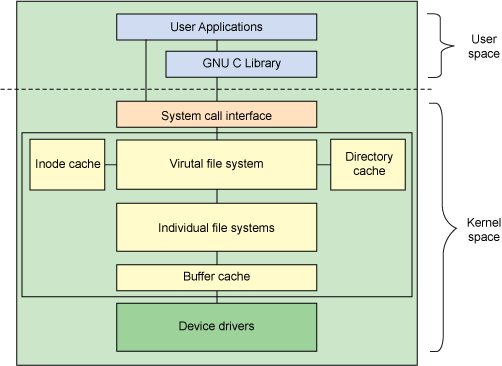
\includegraphics[width=15cm]{theoretical/filesystem-arhitecture.png}
            \end{center}
        \end{figure}

    \subsection{User space}

\section{Git}
    Git is one of the most popular, free and open source, distributed control system. It was originally created by Linus Torvalds with the purpose of improving Linux development which became very cumbersome to maintain, because of the large number of patches that needed to be reviewed and integrated in the kernel.
    
    The central component of git is repository. A repository is a directory which contains all the necessary files which git uses to manage the content and the history. This repository can be bare, containing only the necessary parts, without the content itself, or non-bare with the content.
    
    In order to get a repository on the local system, you need to clone it. You can clone a repository from a local machine or a remote one. Git can use different protocols in order to clone a repository (ssh, http/https or git protocol). Every change that was managed by git can be pushed to a remote repository. Each repository on which you want to push or pull changes has an address and a name. The data structure that encapsulate those attributes is called remote. You can have multiple remotes on a local repository, with different address but with unique local names. The default remote (initially used to clone the repository) is called origin.
    
    Using remotes you can distribute the code and work offline. Changes can be synchronized between multiple remote and any raising conflicts would be solved automatically (if possible).
    
    \subsection{Overview}
        After a remote repository is cloned on the local machine one can start changing it's content. Git will track only the files that are already in the repository. Newly created files needs to be manually add as tracked. Empty directories are not track-able.
        
        Any new change is viewed and tracked by git, but not automatically transformed in a version. In order to group the changes, git uses the concept of stage. Each new change is tracked by git in so called working stage. In this zone, the changes are very volatile. If you want to pull content from a different remote, git will stop you in order to save the local changes. In order to group them, you need to add the changed files to the staging are, by using `git add` command.
        
        Once you group the changes together, by moving the files to the stage area, you can create a version. That version is named commit. A commit is a git object, which contains a group of files that were changed, who did the change, who created the commit and when. Beside those metadata, git will attach an unique hash to it in order to be easily identifiable and a reference to the commit before it, called parent. In this way, git can offer an ordered log (not by time, but the order of changes, because you can rewrite the history and relocate a given commit in it's tree of changes) giving you a broad understanding of the changes which were made.
        
        Given the fact that each commit has a parent, you can easily for a chain of commits, called a branch. You can create as many branches as you want, starting with a commit. The default branch is consider to be master. A branch can be created just locally and pushed to any remote repositories afterwards. The last commit from a given branch is called HEAD.
        You can change the HEAD at any time, changing the state of the local or remote repository.
        
        From a commit two branches can diverge. If you want to bring commits from another branch to a given current branch, you can do that use two methods: rebasing and merging.
        Using the rebase method you will apply the current commits (set of changes) to the last commit of the branch you want to rebase into, in the order of which the commits were created, one by one. Any conflicts will be solved at commit level, when is the case. 
        The merging method will try to apply the changes without to keep track of the order of commits. All conflicts will be solved at the end of the methods and will end with a commit. The safest and cleanest method is the rebase method, but a big inconvenience is that it will rewrite the history, creating new commits (with the same data and metadata: date, author, commiter etc.) for each applied commit.
        
        You can use the any of those methods in order to apply remote changes to current state of the content. Git can manage the branches from all the remotes and using some porcelain commands, you can decide which change to be applied to the local content.
        
        Another useful structure which git offer is tag. A tag is a frozen reference which will point to given commit and has a message and some metadata attach to it. like a commit. The commit to which point can't be change and it has no parent. Tags are used in order to froze the state of a given repository to a commit. 
        
        You can imagine the entire repository like a tree, with multiple branches. The local repository will point to a certain reference. This reference can be a tag, the head of a branch or just the hash of a commit. In this way, you can easily change the state of your repository, by checking-out on different references. The checkout operation can have multiple modes (soft, hard) and in case of conflicts, you can solve them manually or by accepting the local changes (referred as ours) or the remote ones (referred as theirs).
        
    \subsection{Internals}
        Until now we talked about git more from a functional point of view, like a tool. But git can be viewed like a database as well. More precisely like a key-value database. In this way, one can refer to git as a content addressable filesystem. You can add any type of content into it and get back a key which you can use to retrieve the content back. In order to investigate this further we need to take a look at dot git directory.
        
        Dot git directory contains all the data and the meta data of our repository. The part of meta data is stored in the very descriptive file. One of the most important are:
        
        \begin{itemize}
            \item HEAD: the current reference to which your repository points. Usually it will be refs/heads/master
            \item refs: all known references, group by remotes. Here you will also find the mapping between branches and commits.
            \item index: the staging area with it's meta data, like file names, timestamps and hashes of the files managed by git.
        \end{itemize}
        
        \begin{figure}[h]
           \begin{center}
               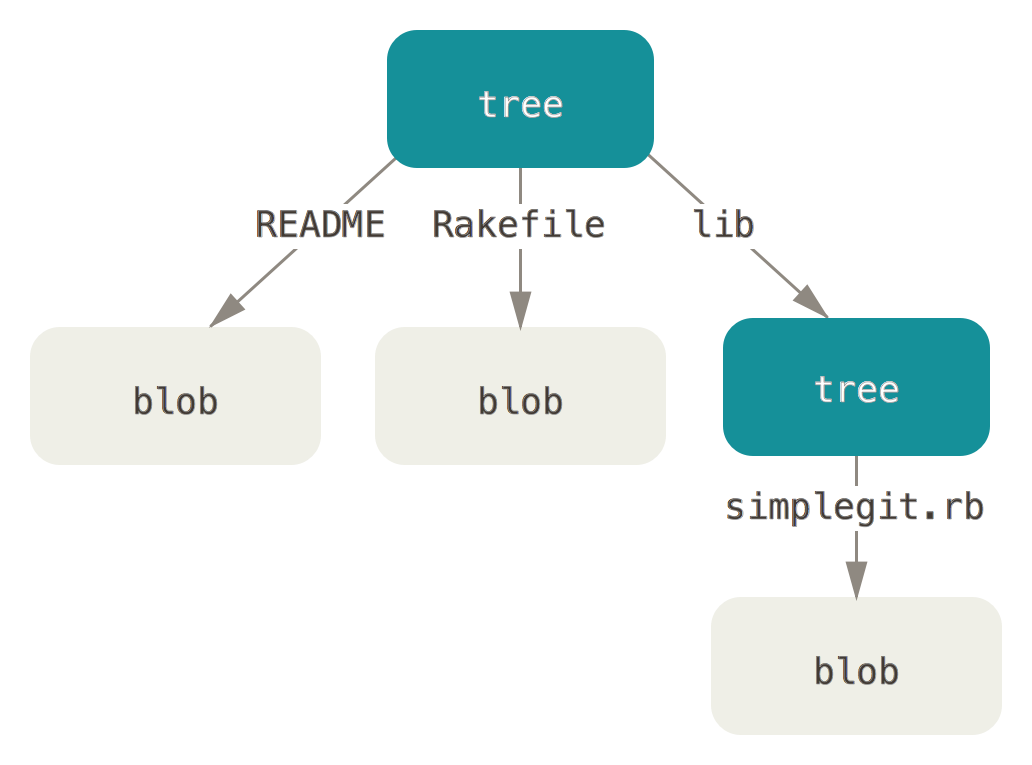
\includegraphics[width=15cm]{technology/data-model-1.png}
            \end{center}
        \end{figure}
    
\section{Python}
    \subsection{About}
    \subsection{CFFI}
    \subsection{fusepy}
    \subsection{libgit2}
    
\section{Similar Projects}
    \subsection{ZFS}